% Source: graduate-coursework/Research/Intro_to_Agents/handouts/Part8_Advanced_Topics.tex

\documentclass[border=4pt]{standalone}
\usepackage[T1]{fontenc}
\usepackage{graphicx}
\usepackage{lmodern}
\usepackage{tikz}
\usepackage{xcolor}
\usetikzlibrary{shapes.geometric, arrows.meta, positioning, calc, fit, backgrounds, matrix, decorations.pathreplacing}

\definecolor{UofSCGarnet}{HTML}{73000a}
\definecolor{UofSCBlack}{HTML}{000000}
\definecolor{UofSCWhite}{HTML}{ffffff}
\definecolor{UofSCRose}{HTML}{CC2E40}
\definecolor{UofSCAtlantic}{HTML}{466A9F}
\definecolor{UofSCCongaree}{HTML}{1F414D}
\definecolor{UofSCHorseshoe}{HTML}{65780B}
\definecolor{UofSCGrass}{HTML}{CED318}
\definecolor{UofSCHoneycomb}{HTML}{A49137}
\definecolor{UofSC90Black}{HTML}{363636}
\definecolor{UofSC70Black}{HTML}{5C5C5C}
\definecolor{UofSC50Black}{HTML}{A2A2A2}
\definecolor{UofSCWarmGrey}{HTML}{676156}
\definecolor{UofSCSandstorm}{HTML}{FFF2E3}
\definecolor{UofSCDarkGarnet}{HTML}{570008}
\definecolor{UofSCAzalea}{HTML}{844247}

\tikzset{
    % Sharp corners for all nodes
    every node/.style={font=\small},
    % Process box style
    process/.style={
        rectangle,
        draw=UofSCBlack,
        fill=UofSCWhite,
        minimum width=2.5cm,
        minimum height=0.8cm,
        align=center,
        font=\footnotesize
    },
    % Decision box style
    decision/.style={
        diamond,
        draw=UofSCBlack,
        fill=UofSCSandstorm,
        minimum width=2cm,
        minimum height=1cm,
        align=center,
        font=\footnotesize,
        aspect=2
    },
    % Start/End style
    startstop/.style={
        rectangle,
        draw=UofSCGarnet,
        fill=UofSCGarnet,
        text=UofSCWhite,
        minimum width=2cm,
        minimum height=0.7cm,
        align=center,
        font=\footnotesize\bfseries
    },
    % Arrow style
    arrow/.style={
        ->,
        >=Stealth,
        thick,
        color=UofSCBlack
    },
    % Failure node
    failure/.style={
        rectangle,
        draw=UofSCRose,
        fill=UofSCRose!20,
        minimum width=2cm,
        minimum height=0.7cm,
        align=center,
        font=\footnotesize
    },
    % Success node
    success/.style={
        rectangle,
        draw=UofSCHorseshoe,
        fill=UofSCHorseshoe!20,
        minimum width=2cm,
        minimum height=0.7cm,
        align=center,
        font=\footnotesize
    },
    % Highlight box
    highlight/.style={
        rectangle,
        draw=UofSCGarnet,
        fill=UofSCGarnet!10,
        line width=1.5pt,
        minimum width=2.5cm,
        minimum height=0.8cm,
        align=center,
        font=\footnotesize
    },
    % Security threat style
    threat/.style={
        rectangle,
        draw=UofSCRose,
        fill=UofSCRose!15,
        minimum width=2.2cm,
        minimum height=0.7cm,
        align=center,
        font=\footnotesize
    },
    % Agent node
    agent/.style={
        rectangle,
        draw=UofSCAtlantic,
        fill=UofSCAtlantic!15,
        minimum width=2.2cm,
        minimum height=0.8cm,
        align=center,
        font=\footnotesize
    },
    % Human node
    human/.style={
        rectangle,
        draw=UofSCCongaree,
        fill=UofSCCongaree!15,
        minimum width=2.2cm,
        minimum height=0.8cm,
        align=center,
        font=\footnotesize
    },
    % Cost node
    cost/.style={
        rectangle,
        draw=UofSCHoneycomb,
        fill=UofSCHoneycomb!20,
        minimum width=2cm,
        minimum height=0.7cm,
        align=center,
        font=\footnotesize
    },
    % Test node
    test/.style={
        rectangle,
        draw=UofSCAtlantic,
        fill=UofSCAtlantic!10,
        minimum width=2cm,
        minimum height=0.7cm,
        align=center,
        font=\footnotesize
    },
    % Pipeline stage
    pipeline/.style={
        rectangle,
        draw=UofSCCongaree,
        fill=UofSCCongaree!10,
        minimum width=2.5cm,
        minimum height=0.8cm,
        align=center,
        font=\footnotesize
    },
    % Timeline event
    timeline/.style={
        rectangle,
        draw=UofSCGarnet,
        fill=UofSCWhite,
        minimum width=1.8cm,
        minimum height=0.6cm,
        align=center,
        font=\tiny
    }
}

\begin{document}
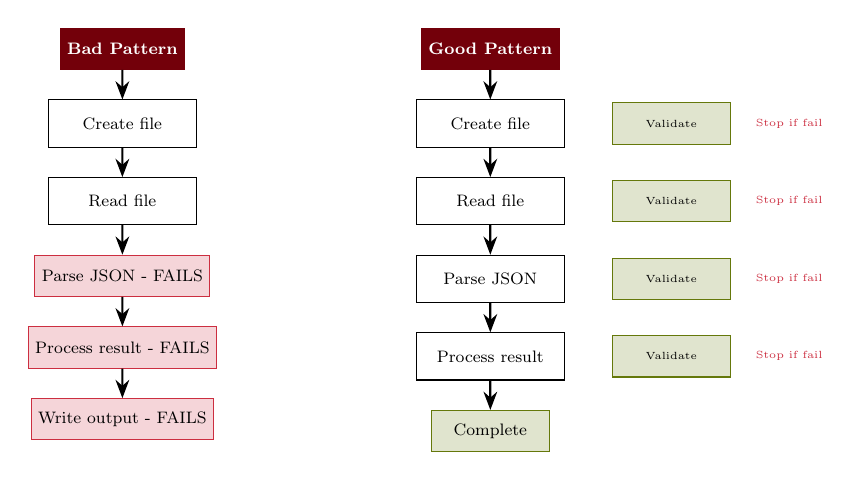
\begin{tikzpicture}[node distance=0.5cm and 1.5cm, scale=0.75, transform shape]
        % Bad pattern
        \node (bad) [startstop] {Bad Pattern};
        \node (b1) [process, below=of bad] {Create file};
        \node (b2) [process, below=of b1] {Read file};
        \node (b3) [failure, below=of b2] {Parse JSON - FAILS};
        \node (b4) [failure, below=of b3] {Process result - FAILS};
        \node (b5) [failure, below=of b4] {Write output - FAILS};

        \draw [arrow] (bad) -- (b1);
        \draw [arrow] (b1) -- (b2);
        \draw [arrow] (b2) -- (b3);
        \draw [arrow] (b3) -- (b4);
        \draw [arrow] (b4) -- (b5);

        % Good pattern
        \node (good) [startstop, right=4cm of bad] {Good Pattern};
        \node (g1) [process, below=of good] {Create file};
        \node (v1) [success, right=0.8cm of g1, font=\tiny] {Validate};
        \node (g2) [process, below=of g1] {Read file};
        \node (v2) [success, right=0.8cm of g2, font=\tiny] {Validate};
        \node (g3) [process, below=of g2] {Parse JSON};
        \node (v3) [success, right=0.8cm of g3, font=\tiny] {Validate};
        \node (g4) [process, below=of g3] {Process result};
        \node (v4) [success, right=0.8cm of g4, font=\tiny] {Validate};
        \node (g5) [success, below=of g4] {Complete};

        \draw [arrow] (good) -- (g1);
        \draw [arrow] (g1) -- (g2);
        \draw [arrow] (g2) -- (g3);
        \draw [arrow] (g3) -- (g4);
        \draw [arrow] (g4) -- (g5);

        % Stop indicators
        \node [font=\tiny\color{UofSCRose}, right=0.3cm of v1] {Stop if fail};
        \node [font=\tiny\color{UofSCRose}, right=0.3cm of v2] {Stop if fail};
        \node [font=\tiny\color{UofSCRose}, right=0.3cm of v3] {Stop if fail};
        \node [font=\tiny\color{UofSCRose}, right=0.3cm of v4] {Stop if fail};
    \end{tikzpicture}
\end{document}
